\documentclass[11pt]{beamer}
\usepackage[utf8]{inputenc}
\usepackage{natbib}
\usepackage{graphicx}

%%%%%%%% tema e cor %%%%%%%%
\mode<presentation> {
\usetheme{Madrid}
%\usecolortheme{albatross}
}

\title{Analysing Gravitational Wave Observation}
\author{Team Birdies}


\author{Team Birdies}
\date{July 5 2019}
\begin{document}
\institute[] % (optional)
{
    \begin{itemsize}
        \item Umar Farooq
        \item Ilgwon Park
        \item Gangmin Park
        \item Cyril Briand
    \end{itemsize}
}

\maketitle



\begin{frame}{LIGO}
\title{Laser Interferometer Gravitational-Wave Observatory}


\begin{figure}[h!]
\centering
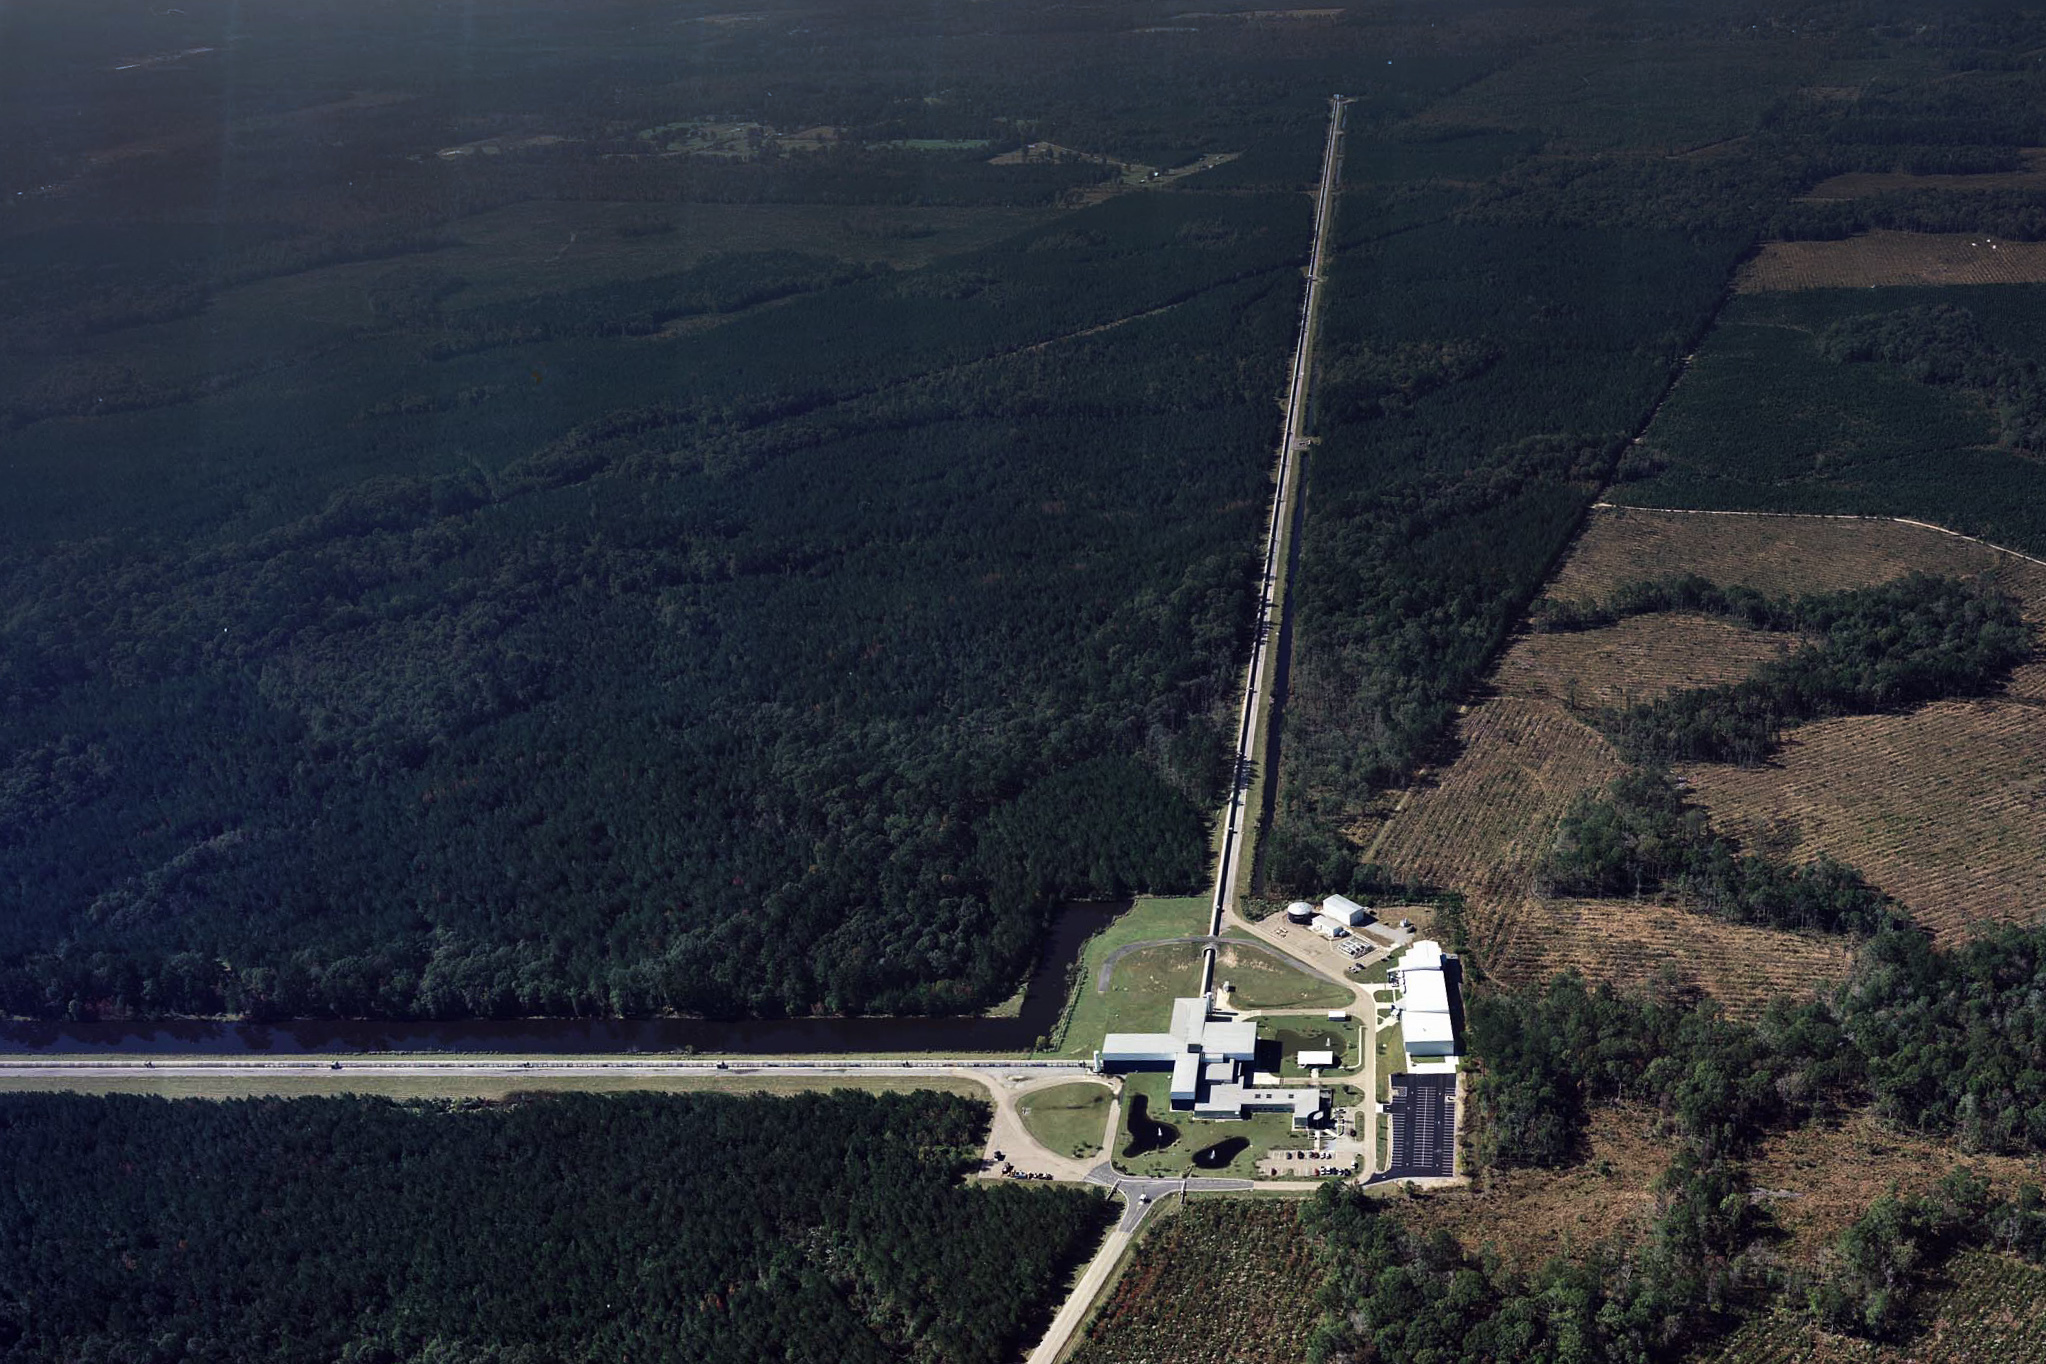
\includegraphics[scale=0.2]{ligo.jpg}
\caption{LIGO Livingston Observatory}
\label{fig:ligo livingston observatory}
\end{figure}

\textbf{Objectives}
\begin{itemize}
    \item Detect cosmic gravitational waves
    \item Make them an observation tool
\end{itemize}
\\
\textbf{Achievement}
\begin{itemize}
    \item Detected multiple binary black hole mergers
    \item Detected binary neutron star
\end{itemize}
\end{frame}


\begin{frame}{Why are we doing this project}
\begin{itemize}
\setlength\itemsep{1em}
\item Pilot project to learn about scientific software
\item Well documented HPC project
\item Intro to statistical analysis
\item Opportunity to document and suggest improvements 
\end{itemize}
\end{frame}

\section{Jupyter Notebook}
\begin{frame}{Jupyter Notebook}
\begin{block}{Definition}
The Jupyter Notebook is an open-source web application that allows you to create and share documents that contain live code, equations, visualizations and narrative text.
\end{block}

\begin{block}{Usage}
Data cleaning and transformation, numerical simulation, statistical modeling, data visualization, machine learning, and much more.
\end{block}

\end{frame}
\begin{frame}{Jupyter Notebook}
\begin{block}{Anaconda}
Regardless of OS types, Anaconda supports Jupyter notebook including python and scientific packages such as numpy, Scipy and pandas. \\ This way is highly recommended.
\end{block}

\begin{block}{pip}
User can install Jupyter by just pip like below \\
python3 -m pip install --upgrade pip \\
python3 -m pip install jupyter
\end{block}

\end{frame}
\begin{frame}{Jupyter Notebook}
    
\begin{figure}
    \centering
    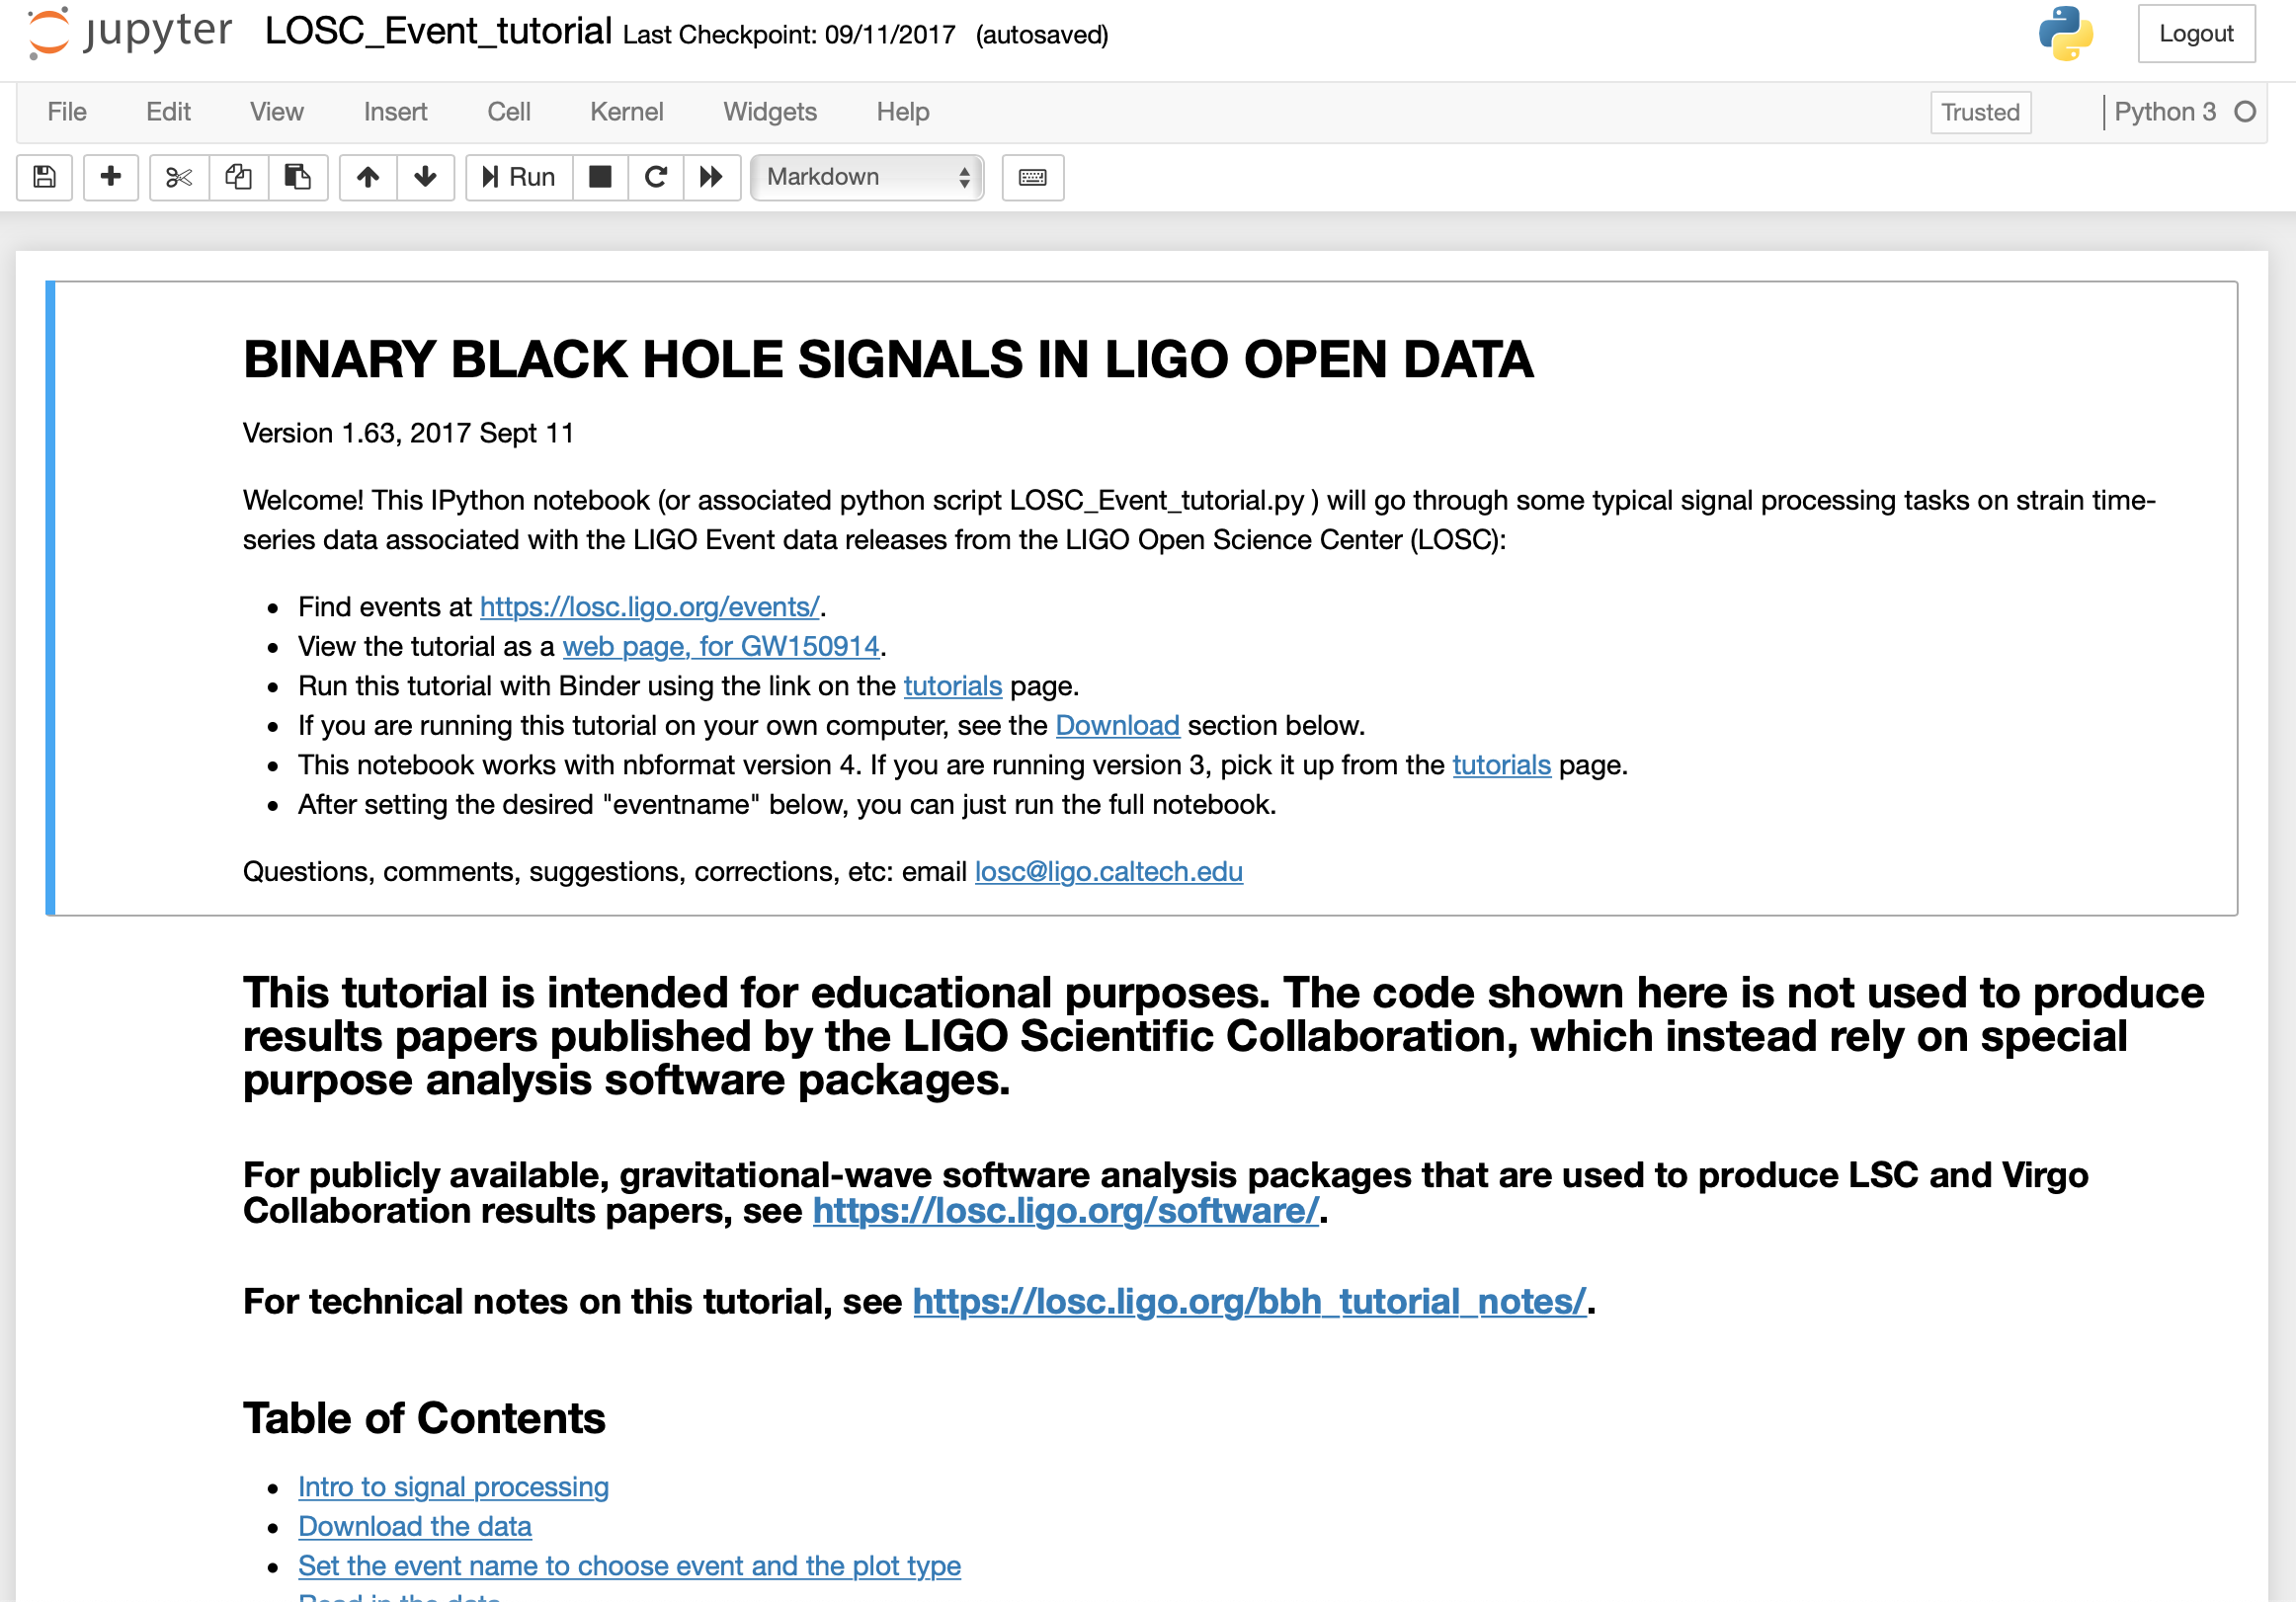
\includegraphics[width=.7\textwidth]{img/jupyter_losc_intro.png}
    \caption{Applying project to Jupyter Notebook}
    % \label{fig:my_label}
\end{figure}

\end{frame}
\begin{frame}{Jupyter Notebook}
    
\begin{figure}
    \centering
    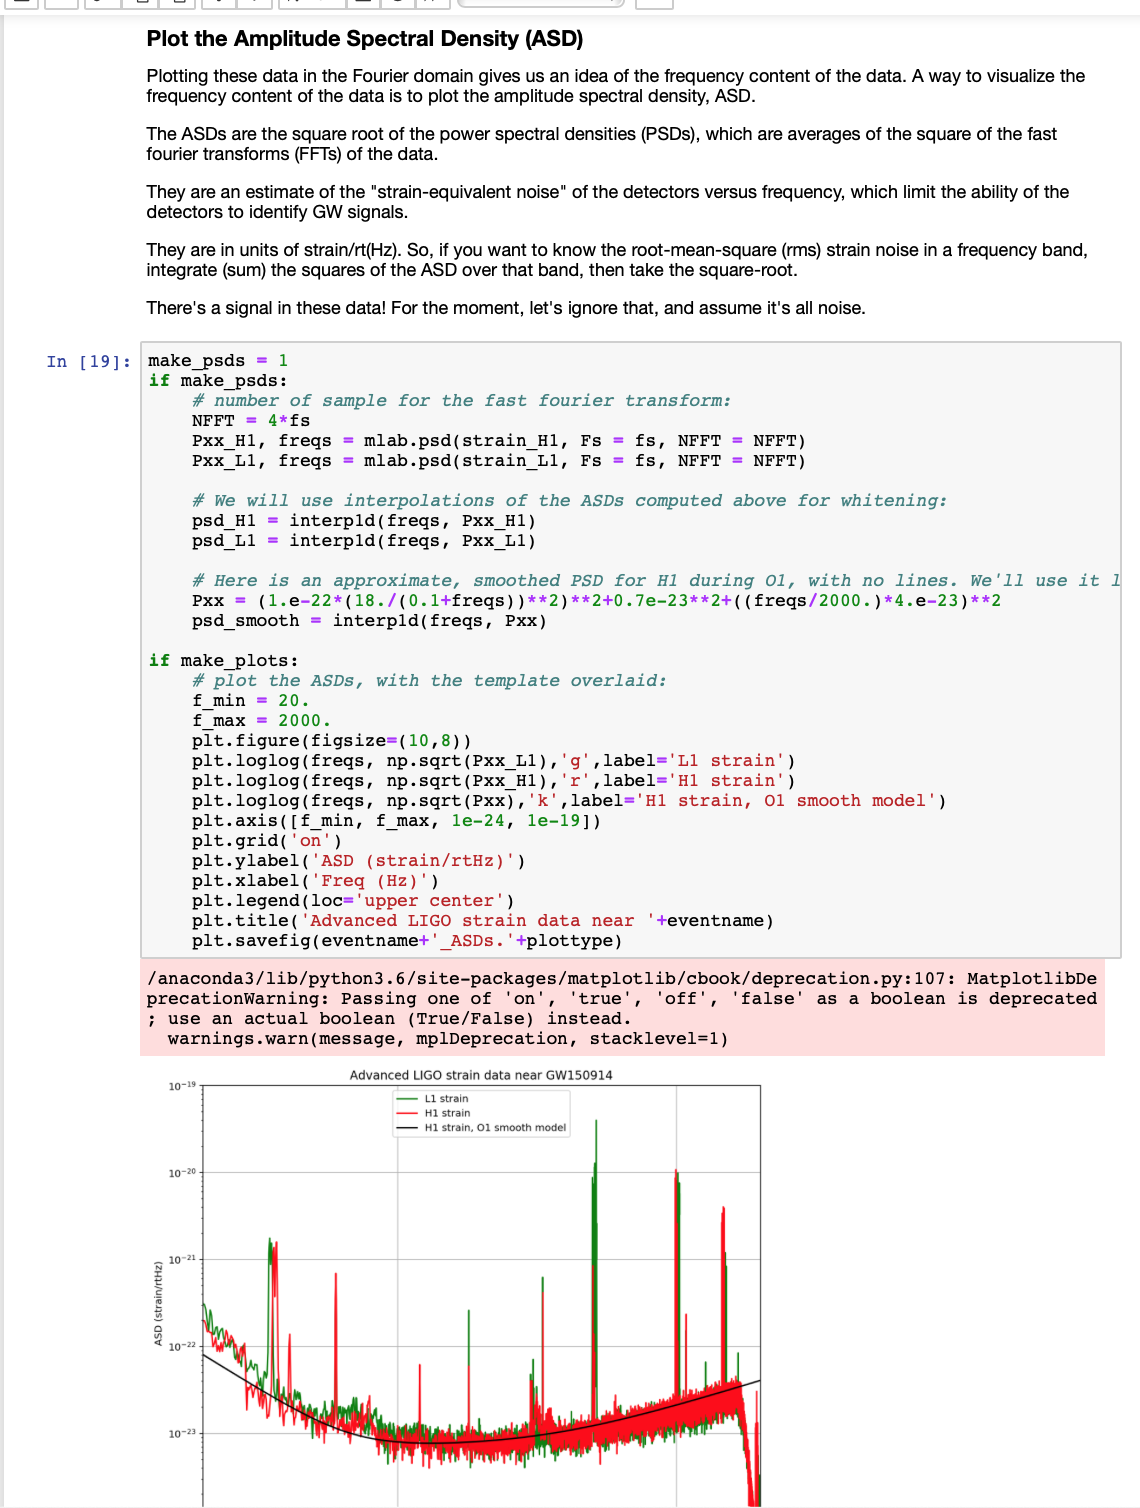
\includegraphics[width=.4\textwidth]{img/jupyter_losc_intro2.png}
    \caption{Applying project to Jupyter Notebook}
\end{figure}

\end{frame}

\begin{frame}{What we are going to}
\textbf{the direction of our study}\\
We're going to go through the process of detecting gravitational waves and converting them into audio files through some sample data from the paper.\\
\textbf{the point of our attention..}
\\
\begin{block}{Hypothesis}
Parameters required for frequency analysis for gravitational wave detection will affect the results in certain directions.
\end{block}
\begin{block}{proof process}
\begin{itemsize}
\begin{enumerate}
    \item Compare the magnitude of gravitational waves between different samples
    \item Get the relationship of gravitational waves according to parameters. 
\end{enumerate}

\end{itemsize}
\end{block}
\end{frame}

\begin{frame}{Sample data & parameters}
    \textbf{we have 4 BBH events}
    \begin{figure}[!t]
    
\includegraphics[width = 0.3\columnwidth]{data.PNG}
    \end{figure}
    \textbf{parameters}\\
    \usepackage{example of GW150914}
    \begin{figure}[!t]
    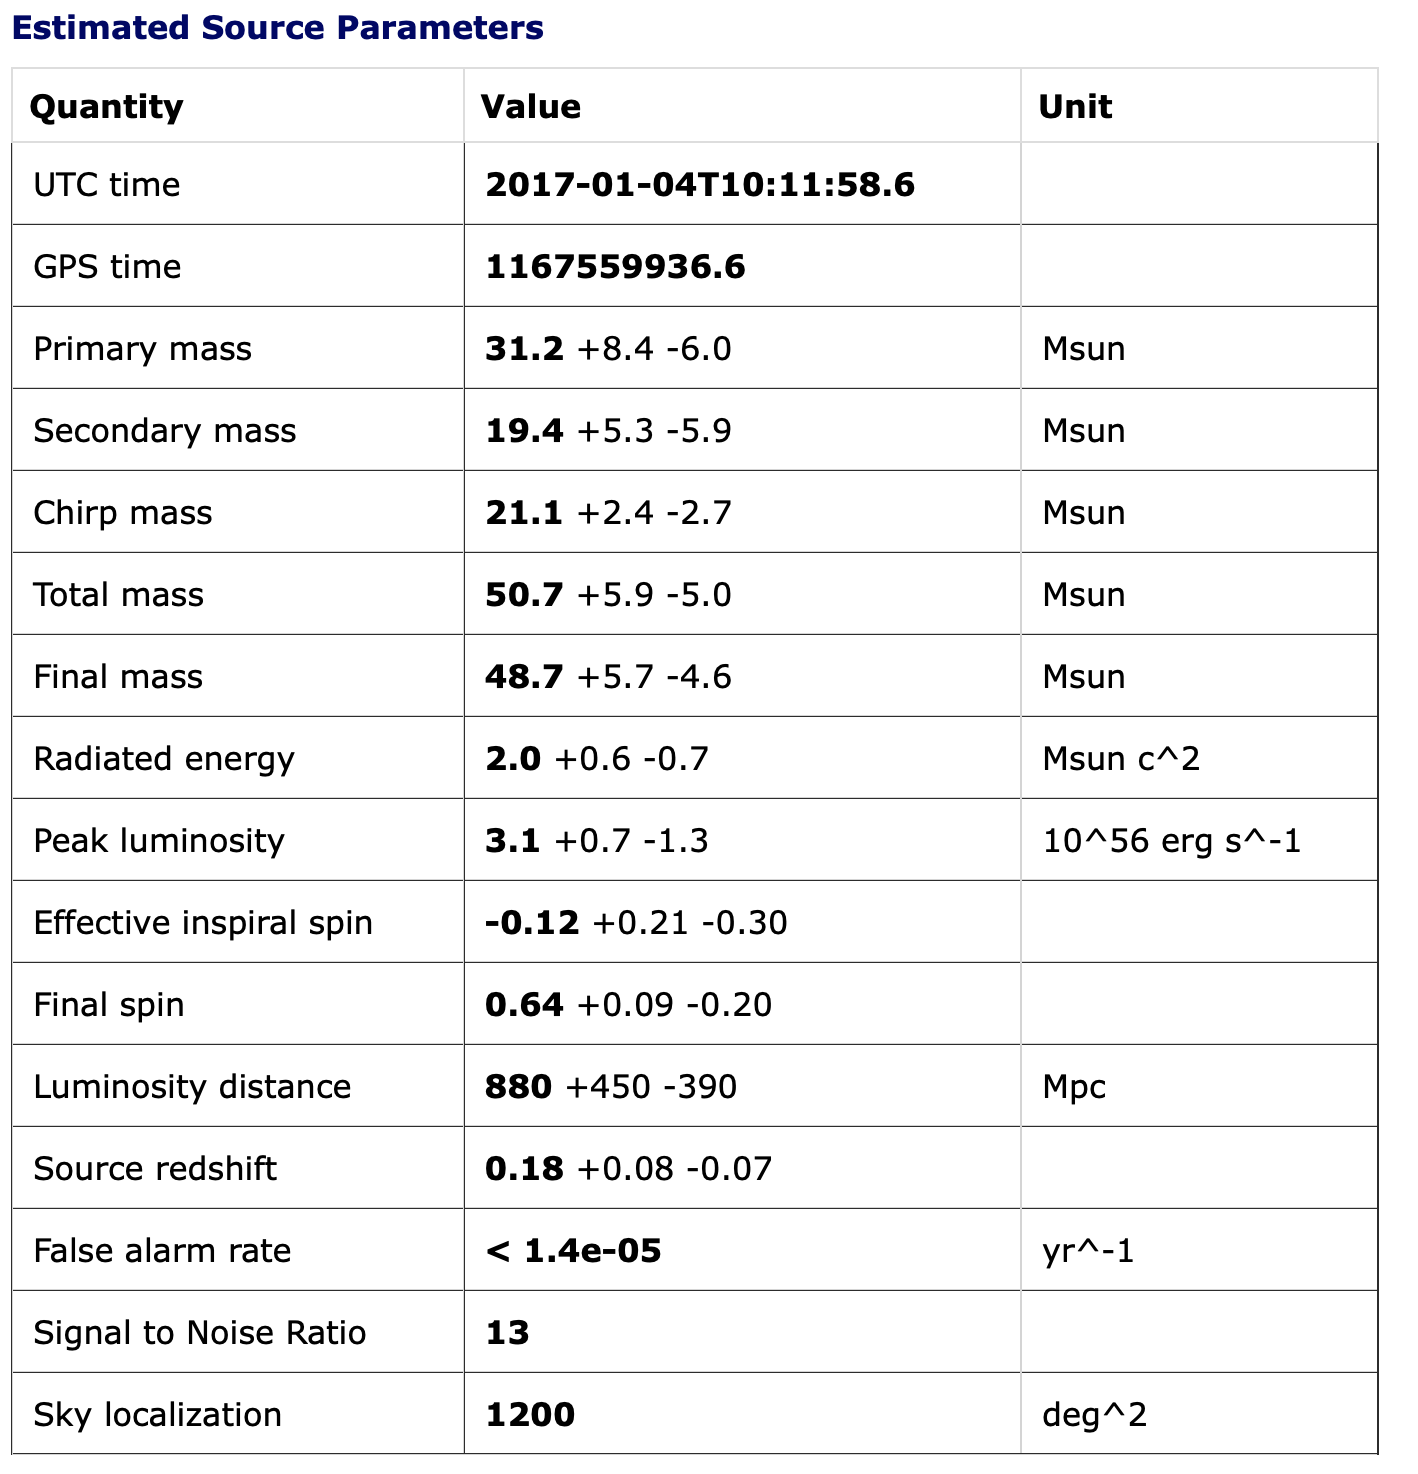
\includegraphics[width = 0.4\columnwidth]{prameters.png}
    \end{figure}
\end{frame}

\begin{frame}{Questions}
    \begin{figure}[!t]
    
\includegraphics[width = 0.9\columnwidth]{questions.jpg}
    \end{figure}
\end{frame}

\end{document}


